\documentclass[conference]{IEEEtran}
\IEEEoverridecommandlockouts
\usepackage{cite}
\usepackage{amsmath}
\usepackage{graphicx}
\usepackage{booktabs}
\usepackage{multirow}
\usepackage{xcolor}
\usepackage[hidelinks]{hyperref}
\usepackage{url}

\begin{document}

\title{Comments First, Weights Matter: A Multitask CodeBERT for Joint Vulnerability and SATD Detection}

\author{\IEEEauthorblockN{Mark Amgad (Student ID: 202610354)}
\IEEEauthorblockA{Master of Software, College of Engineering, Al Ain University, UAE\\
Course 0103613 Requirements Engineering and Architectural Design --- Research Project, Track B1}}

\maketitle

\begin{abstract}
Self-admitted technical debt (SATD) and vulnerabilities are two signals of low internal quality that reviewers want flagged early, and the NLBSE'27 tool competition asks for one model that detects both in a C/C++ function. We study a multitask CodeBERT with three changes to the official baseline: the function's comments are placed before the code in the input, the loss is class-weighted, and each label gets its own decision threshold. On the public test split (30,655 functions) the model reaches a mean F1 of 0.923 against 0.910 for the reproduced baseline (bootstrap 95\% CI of the gain: [0.006, 0.022]). The gain comes entirely from SATD (F1 0.922 vs.\ 0.881, McNemar $p<10^{-5}$), while vulnerability detection is slightly worse after one epoch (0.925 vs.\ 0.939). An ablation over three seeds shows that the class-weighted loss is what makes SATD learnable from limited data; comment placement and threshold tuning add little, and tuned thresholds did not transfer from validation to test. Error analysis shows that most remaining SATD errors occur in functions without any comment, which points to labels derived from comments outside the model's input.
\end{abstract}

\begin{IEEEkeywords}
self-admitted technical debt, vulnerability detection, multitask learning, CodeBERT, NLBSE
\end{IEEEkeywords}

\section{Introduction}
Technical debt that developers admit in comments (SATD) is most often design or requirement debt~\cite{maldonado2017}, so it marks places where a system already deviates from its intended architecture or from its requirements. Vulnerabilities violate a security quality attribute. Both are cheap to act on when found early and costly when they accumulate, and prior work suggests the two co-occur~\cite{russo2025}. A single model that flags both gives a reviewer two quality signals from one pass over a function.

The NLBSE'27 tool competition~\cite{nlbse27} frames this as a multitask problem on MADE-WIC~\cite{madewic}: given a normalized function with its comments, predict \emph{[vulnerability, SATD]}. The official baseline fine-tunes CodeBERT~\cite{codebert} with a shared encoder and a two-output head. We ask:

\textbf{RQ1.} How do a classical TF-IDF model, the official baseline and our multitask variant compare on joint vulnerability and SATD detection?
\textbf{RQ2.} Which of our three changes (comments-first input, class-weighted loss, per-label thresholds) contributes to the result?
\textbf{RQ3.} What kinds of functions does the model still misclassify?

\textbf{Contributions:} (i) a multitask variant that beats the reproduced baseline on mean F1 at the same model size; (ii) a three-seed ablation that isolates the class-weighted loss as the decisive change for SATD; (iii) an error analysis linking residual SATD errors to comments missing from the input; (iv) an open, cached Colab notebook and repository that reproduce every number.

\section{Related Work}
\textbf{SATD detection.} Potdar and Shihab introduced SATD and found it in 2.4--31\% of files of the studied projects~\cite{potdar2014}. Maldonado et al.\ detected design and requirement SATD with a maximum-entropy classifier~\cite{maldonado2017}, and Ren et al.\ used a CNN to improve cross-project performance and explain predictions through key phrases~\cite{ren2019}. These works classify comments; here SATD is predicted at function level from code and comments together.

\textbf{Vulnerability detection.} Devign~\cite{devign} and Big-Vul~\cite{bigvul} provide function-level C/C++ datasets; MADE-WIC fuses them with SATD annotations~\cite{madewic}. Chakraborty et al.\ showed that deep models lose much of their reported performance on realistic data~\cite{chakraborty2022}, and Croft et al.\ found 20--71\% of vulnerability labels inaccurate and many duplicates in such datasets~\cite{croft2023}, which motivates our leakage checks and label-noise discussion.

\textbf{Multitask learning.} Multitask learning shares a representation across related tasks~\cite{caruana1997}. Russo et al.\ compared single- and multitask CodeBERT (VulSATD) on MADE-WIC and found no significant difference, even with a weighted loss~\cite{russo2025}. We keep the multitask setting fixed and instead study input construction, loss weighting and thresholds under the competition protocol, with statistical tests against the official baseline.

\section{Dataset and Approach}
\subsection{Dataset}
The competition data (Hugging Face \url{NLBSE/nlbse27-code-comment-classification}, derived from MADE-WIC, CC BY 4.0) has 214,586 training and 30,655 public test functions from 15 projects; the hidden test split is held by the organizers. 32.8\% of functions are vulnerable, 1.65\% carry SATD and 1.09\% both, so 66\% of SATD functions are also vulnerable, against 33\% overall. Only 14.2\% of functions contain any comment; \emph{todo}, \emph{fixme} and \emph{xxx} appear in 34\%, 27\% and 21\% of SATD comments and almost never elsewhere.

\textbf{Cleaning and splits.} We hold out 10\% of the training split as validation, stratified on the joint label with seed 42 (193,127 / 21,459). We found 808 exact duplicate functions inside training and 251 test functions (0.82\%) that also occur in training. All new models are trained on 192,125 rows with duplicates and any overlap with validation or test removed; every approach is also scored on a \emph{clean} test subset without the overlapping functions. The test split is used once, for final scoring; all thresholds are chosen on validation.

\subsection{Approaches}
\textbf{A1: TF-IDF + LR.} Identifier unigrams and bigrams (300,000 features, sublinear TF) and one class-balanced logistic regression per label.

\textbf{A2: Official baseline.} The organizers' trained \texttt{codebert-base} model with a two-output head, input = code only, threshold 0.5. We re-scored it ourselves (reproduction).

\textbf{A3: Ours.} The same architecture (CodeBERT, 125M parameters, shared encoder, two sigmoid outputs) with three changes. \emph{(a) Comments first:} all \texttt{//} and \texttt{/* */} comments are extracted with a regular expression (capped at 1,000 characters) and fed as the first segment of a sentence pair, \texttt{<s> comments </s></s> code </s>}, with \texttt{longest\_first} truncation at 512 tokens so the code is cut before the comments. \emph{(b) Class-weighted loss:} binary cross-entropy in which positives of label $j$ are weighted by $w_j=\sqrt{N_j^-/N_j^+}$, giving $w=1.43$ (vulnerability) and $w=7.72$ (SATD). \emph{(c) Per-label thresholds}, chosen on validation from $\{0.02,0.04,\dots,0.94\}$ to maximize each label's F1.

\textbf{Setup.} AdamW, learning rate $2\cdot10^{-5}$, weight decay 0.01, 6\% linear warm-up, batch 16, fp16, one epoch (12,071 steps, 80 min on one Colab T4). Metrics: per-label precision, recall, F1, macro-F1, MCC and PR-AUC; the competition metric is the mean of the two F1 scores. We compare paired predictions with McNemar's test~\cite{dietterich1998} and give 95\% bootstrap intervals (1,000 resamples) for differences in mean F1. The ablation (RQ2) trains variants on a stratified 10\% sample of the clean training rows (19,212 functions, a new sample per seed) with seeds 42--44, tunes thresholds on a fixed 5,000-function validation sample, and scores the full test split.

\section{Results and Discussion}
\begin{table*}[t]
\centering
\caption{Public test split (30,655 functions). Thresholds tuned on validation unless stated. Best F1 per column in bold.}
\label{tab:main}
\begin{tabular}{lcccccccccc}
\toprule
 & & \multicolumn{4}{c}{Vulnerability} & \multicolumn{4}{c}{SATD} & \\
\cmidrule(lr){3-6}\cmidrule(lr){7-10}
Approach & Thresholds & P & R & F1 & MCC & P & R & F1 & MCC & Mean F1 \\
\midrule
A1 TF-IDF + LR & 0.48 / 0.76 & .694 & .809 & .748 & .614 & .920 & .796 & .854 & .854 & .801 \\
A2 Official baseline & 0.50 / 0.50 & .943 & .935 & \textbf{.939} & .909 & .978 & .802 & .881 & .884 & .910 \\
A2 Official baseline, tuned & 0.34 / 0.02 & .942 & .936 & \textbf{.939} & .909 & .978 & .802 & .881 & .884 & .910 \\
A3 Ours, threshold 0.5 & 0.50 / 0.50 & .924 & .926 & .925 & .888 & .987 & .877 & \textbf{.929} & .929 & \textbf{.927} \\
A3 Ours (full method) & 0.50 / 0.04 & .924 & .926 & .925 & .888 & .971 & .877 & .922 & .922 & .923 \\
\bottomrule
\end{tabular}
\end{table*}

\subsection{RQ1: Comparison of approaches}
Table~\ref{tab:main} shows that our full method reaches a mean F1 of 0.923, 0.013 above the official baseline, whose reported scores (0.939 / 0.881 / 0.910) we reproduce exactly. The bootstrap interval of the gain is [0.006, 0.022]. The two tasks move in opposite directions. On SATD our model is right where the baseline is wrong 42 times and the reverse 8 times (McNemar $\chi^2=21.8$, $p=3.1\cdot10^{-6}$); recall rises from 0.802 to 0.877 and PR-AUC from 0.817 to 0.890, so the gain is not a threshold artifact. On vulnerability the baseline is better (716 vs.\ 429 discordant pairs, $p<10^{-16}$), likely because we trained for a single epoch. TF-IDF trails both transformers by 0.11--0.12 mean F1 ($p<10^{-10}$ for both tasks), though its SATD F1 of 0.854 confirms how lexical SATD is. Removing the 251 overlapping test functions changes no score by more than 0.001, so leakage does not explain the results.

\subsection{RQ2: Ablation}
\begin{figure}[t]
\centering
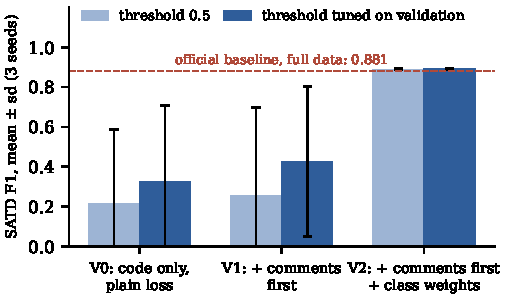
\includegraphics[width=\columnwidth]{figures/ablation_satd.pdf}
\caption{Ablation on 10\% of the training data, three seeds. Without class weights, SATD F1 collapses in most seeds.}
\label{fig:ablation}
\end{figure}

\begin{table}[t]
\centering
\caption{Ablation, mean $\pm$ sd over seeds 42--44 (10\% training data, full test split). Each variant adds to the one above it.}
\label{tab:ablation}
\footnotesize\setlength{\tabcolsep}{3pt}
\begin{tabular}{llccc}
\toprule
Variant & Thr. & Vuln.\ F1 & SATD F1 & Mean F1 \\
\midrule
V0 code only & 0.5 & .824$\pm$.008 & .215$\pm$.373 & .519$\pm$.190 \\
 & tuned & .821$\pm$.009 & .325$\pm$.382 & .573$\pm$.196 \\
V1 + comments first & 0.5 & .823$\pm$.009 & .256$\pm$.443 & .539$\pm$.225 \\
 & tuned & .823$\pm$.010 & .426$\pm$.376 & .624$\pm$.193 \\
V2 + class weights & 0.5 & .823$\pm$.017 & .889$\pm$.002 & .856$\pm$.008 \\
 & tuned & .823$\pm$.019 & .891$\pm$.004 & .857$\pm$.010 \\
\bottomrule
\end{tabular}
\end{table}

Table~\ref{tab:ablation} and Fig.~\ref{fig:ablation} isolate the three changes. The class-weighted loss is decisive: with 19,212 training functions (about 320 SATD positives), the unweighted variants learned to predict almost no SATD in two of three seeds, giving SATD F1 0.22--0.26 with standard deviations near 0.4, while the weighted variant reached 0.889 $\pm$ 0.002, above the full-data baseline. Comments-first input adds 0.04 (threshold 0.5) to 0.10 (tuned) SATD F1, well inside the seed variance; we did not test weights without comments-first, so its effect on top of weighting is not measured. Threshold tuning partly rescues the unweighted variants but adds only 0.002 to the weighted one. On the full model, the tuned SATD threshold (0.04) even cost 7 correct predictions on test compared with 0.5 (McNemar $p=0.023$; mean F1 $-0.003$, CI [$-0.006$, $-0.001$]): with only 350 SATD positives in validation, a low threshold overfits. Vulnerability F1 does not depend on any change.

\subsection{RQ3: Error analysis}
Errors concentrate in long inputs: functions longer than 512 tokens (10.6\% of test) have a vulnerability error rate of 11.7\% against 4.1\% for the rest, and a SATD error rate of 0.62\% against 0.20\%. Of the 75 SATD errors (62 misses, 13 false alarms), about 47 occur in functions with no comment at all, and only one miss contains a \emph{todo}-style keyword. We inspected 30 random errors (15 per task):

\begin{itemize}
\item \textbf{SATD label without any comment in the input} (10 of 14 SATD misses). MADE-WIC also annotates leading comments preceding a function~\cite{madewic}, which the competition input does not contain, so these labels are unrecoverable from the input.
\item \textbf{Implicit debt without keywords} (4 misses), e.g., ``new problem now bump the values \dots\ patched up command''.
\item \textbf{Likely label noise} (1 SATD false alarm reading ``hard code the offset for now'', and 3 vulnerability false alarms at probability $\geq$0.99), consistent with the label error rates reported for these sources~\cite{croft2023}.
\item \textbf{Truncation} (6 of 15 vulnerability errors exceed 512 tokens) and \textbf{missing context} (2 misses in functions under 100 tokens, where the flaw presumably depends on callers).
\end{itemize}

\textbf{Cost.} Our input is slightly longer than the baseline's, raising compute from 38.5 to 39.3 GFLOPs per function (+2.2\%) and inference from 7.75 to 8.06 ms per function on a T4 (batch 64, fp16). TF-IDF needs 55 s of training and 0.10 ms per function, a useful floor where cost matters more than accuracy.

\section{Threats to Validity}
\textbf{Internal.} The main model was trained once (one epoch, seed 42); the baseline's training budget is not reported, which may explain the vulnerability gap. The ablation uses 10\% of the data, so effects at full scale may be smaller. \textbf{Construct.} Labels come from automatic and fused annotations and contain noise~\cite{croft2023}; SATD labels can depend on comments absent from the input; F1 depends on thresholds, which is why we also report PR-AUC. \textbf{External.} Results cover C/C++ functions from 15 projects and the public test split only; the hidden test split may differ. \textbf{Conclusion.} Three seeds give coarse variance estimates; McNemar tests are per task, but all reported $p$-values stay significant under a Bonferroni correction for the eight tests run except the threshold comparison ($p=0.023$).

\section{Conclusion and Future Work}
A multitask CodeBERT that weights its rare SATD positives beats the official baseline on mean F1 at the same size and nearly the same cost; the weighting, not the input layout or tuned thresholds, carries the gain. The main obstacles left are label provenance (SATD in comments outside the function) and long functions. Next steps are training for more epochs to close the vulnerability gap, feeding leading comments where available, and handling long functions with sliding windows. Code and notebook: \url{https://github.com/MarkAmgad1/nlbse27-multitask-satd-vuln} and \url{https://colab.research.google.com/drive/1YI0NAOlEyXxoHPA7qPMk_evr-rAmUBOU}.

\section*{Statements}
\textbf{Use of generative AI.} An AI assistant (Claude, Anthropic) was used to help write and debug the notebook and to draft and edit this paper. The author ran all experiments, checked every number against the notebook outputs, and takes responsibility for the content.
\textbf{Data and code availability.} The dataset is public on Hugging Face (MADE-WIC, CC BY 4.0). The notebook, cached results, and paper sources are in the repository above (release \texttt{v1.0-submission}). Code reuses the official baseline's model and task definition~\cite{nlbse27}.

\begin{thebibliography}{00}
\bibitem{nlbse27} M. Mock, T. Borsani, and B. Russo, ``The NLBSE'27 tool competition and challenge,'' in \emph{Proc. 6th Int. Workshop on Natural Language-based Software Engineering (NLBSE)}, co-located with ICSE, 2027. [Online]. Available: \url{https://conf.researchr.org/home/icse-2027/nlbse-2027}
\bibitem{madewic} M. Mock, J. Melegati, M. Kretschmann, N. E. D\'iaz Ferreyra, and B. Russo, ``MADE-WIC: Multiple annotated datasets for exploring weaknesses in code,'' in \emph{Proc. 39th IEEE/ACM Int. Conf. Automated Software Engineering (ASE)}, 2024, pp. 2346--2349, doi: 10.1145/3691620.3695348.
\bibitem{russo2025} B. Russo, J. Melegati, and M. Mock, ``Leveraging multi-task learning to improve the detection of SATD and vulnerability,'' in \emph{Proc. IEEE/ACM 33rd Int. Conf. Program Comprehension (ICPC)}, 2025, doi: 10.1109/ICPC66645.2025.00017.
\bibitem{codebert} Z. Feng \emph{et al.}, ``CodeBERT: A pre-trained model for programming and natural languages,'' in \emph{Findings of the Association for Computational Linguistics: EMNLP 2020}, 2020, pp. 1536--1547.
\bibitem{potdar2014} A. Potdar and E. Shihab, ``An exploratory study on self-admitted technical debt,'' in \emph{Proc. IEEE Int. Conf. Software Maintenance and Evolution (ICSME)}, 2014, pp. 91--100, doi: 10.1109/ICSME.2014.31.
\bibitem{maldonado2017} E. da S. Maldonado, E. Shihab, and N. Tsantalis, ``Using natural language processing to automatically detect self-admitted technical debt,'' \emph{IEEE Trans. Softw. Eng.}, vol. 43, no. 11, pp. 1044--1062, 2017, doi: 10.1109/TSE.2017.2654244.
\bibitem{ren2019} X. Ren, Z. Xing, X. Xia, D. Lo, X. Wang, and J. Grundy, ``Neural network-based detection of self-admitted technical debt: From performance to explainability,'' \emph{ACM Trans. Softw. Eng. Methodol.}, vol. 28, no. 3, art. 15, 2019, doi: 10.1145/3324916.
\bibitem{devign} Y. Zhou, S. Liu, J. Siow, X. Du, and Y. Liu, ``Devign: Effective vulnerability identification by learning comprehensive program semantics via graph neural networks,'' in \emph{Advances in Neural Information Processing Systems (NeurIPS)}, 2019.
\bibitem{bigvul} J. Fan, Y. Li, S. Wang, and T. N. Nguyen, ``A C/C++ code vulnerability dataset with code changes and CVE summaries,'' in \emph{Proc. 17th Int. Conf. Mining Software Repositories (MSR)}, 2020, pp. 508--512.
\bibitem{chakraborty2022} S. Chakraborty, R. Krishna, Y. Ding, and B. Ray, ``Deep learning based vulnerability detection: Are we there yet?'' \emph{IEEE Trans. Softw. Eng.}, vol. 48, no. 9, pp. 3280--3296, 2022.
\bibitem{croft2023} R. Croft, M. A. Babar, and M. M. Kholoosi, ``Data quality for software vulnerability datasets,'' in \emph{Proc. IEEE/ACM 45th Int. Conf. Software Engineering (ICSE)}, 2023, doi: 10.1109/ICSE48619.2023.00022.
\bibitem{caruana1997} R. Caruana, ``Multitask learning,'' \emph{Machine Learning}, vol. 28, no. 1, pp. 41--75, 1997.
\bibitem{dietterich1998} T. G. Dietterich, ``Approximate statistical tests for comparing supervised classification learning algorithms,'' \emph{Neural Computation}, vol. 10, no. 7, pp. 1895--1923, 1998.
\end{thebibliography}

\end{document}
